\chapter{Contract Net}\label{ch:contract_net}

O \textit{Contract Net} é um protocolo que atende aos critérios definidos para caracterizar-se como padrão arquitetural organizacional. Trata-se de um protocolo para comunicação entre agentes voltado ao controle distribuído de tarefas em execução envolvendo negociação entre agentes. Seu detalhamento, enquanto padrão, é realizado a seguir, baseando-se no protocolo de comunicação \textit{FIPA-Contract-Net}. Para maior entendimento dos atos comunicativos FIPA, a Seção \ref{subsubsec:fipa_acl} busca descrever os mesmos.



\begin{description}
  \item[Nome do padrão:] \textit{Contract Net}.
    \item[Referências:]    \citeonline[pág. 23]{developing}, \citeonline[pág. 31]{jadeguide}.
    \item[Categoria:] \textit{Bureaucracy structure}.
    \item[Problema:] um agente, o \initiator (ou iniciador), que deseja ter alguma tarefa executada por um ou mais agentes, os \textit{Responders} (ou participantes), e ainda deseja otimizar uma função que caracteriza a tarefa. Esta função é comumente expressa, por exemplo, como custo, tempo até a conclusão, e a distribuição justa das tarefas \cite{developing}.
    \item[Solução:] para uma determinada tarefa, qualquer número de participantes pode responder com uma proposta; os demais devem recusar. As negociações prosseguem com os Participantes que propuseram.
O Iniciador solicita um número \textit{m} de propostas de outros agentes através da emissão de um convite à apresentação de propostas (\textit{Call for Proposals}), que especifica a tarefa e quaisquer condições que o Iniciador coloca sobre a execução da tarefa. 

Os participantes que recebem o convite à apresentação de propostas são vistos como potenciais contratados e são capazes de gerar um número \textit{n} de respostas. Destes, \textit{j} são o número de propostas para realizar a tarefa, especificada como proposta.

A proposta do Participante inclui as pré-condições que o Participante está definindo para a tarefa, que pode ser o preço, o tempo em que a tarefa será feita, dentre outras. Alternativamente, os Participantes podem se recusar a propor. Uma vez passado o prazo, o Iniciador avalia o valor recebido


    \item[Protocolos associados:] o \textit{FIPA-Contract-Net} está associado a este padrão e pode ser representado pela Figura \ref{fig:contract_net_protocol}.

    \begin{figure}[!htb]
        \centering
        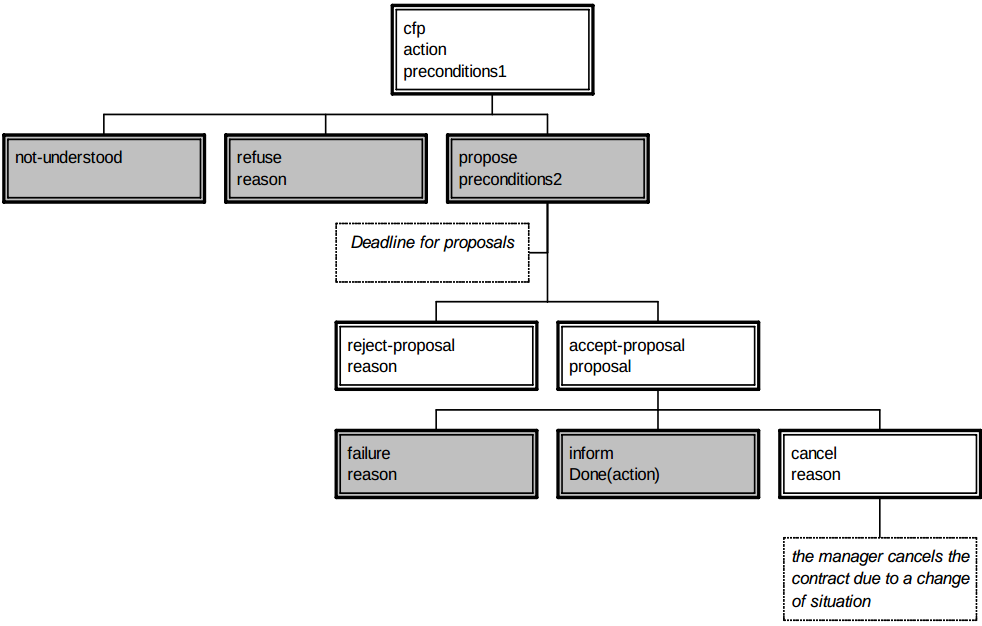
\includegraphics[scale=0.4]{figuras/contract-net-protocol.png}
        \caption{Protocolo de Interação \textit{FIPA-Contract-Net}. Fonte: \citeonline[pág. 36]{jadeguide}}
        \label{fig:contract_net_protocol}
    \end{figure}

O \textit{FIPA-Contract-Net} permite que o \initiator envie um \textit{Call for Proposal} (CFP) a um conjunto de \textit{Responders}, avalie suas propostas e, por fim, realize sua escolha aceitando uma das propostas ou até mesmo rejeitando a todas \cite{jadeguide}.

A mensagem CFP contém a ação a ser realizada e, se necessário, condições de execução. Os \textit{Responders} podem responder com as seguintes mensagens: \textit{Propose} - sua proposta composta por pré-condições, custo e tempo -, \textit{Refuse} para recusa - ou \textit{Not-Understood} em caso de falhas de comunicação. 

Após avaliar todas as propostas, o \initiator realiza sua escolha e informa quais foram rejeitadas e quais foram aceitas (através da mensagem \textit{Accept Proposal}). Estes, assim que completam suas tarefas, respondem com \textit{Inform} o resultado de sua ação - como finalizada ou como \textit{Failure}.

O \initiator pode decidir cancelar o protocolo, enviando uma mensagem \textit{Cancel}, antes da ação ter sido realizada e a última mensagem ter sido recebida.


O \textit{FIPA-Contract-Net} é implementado por dois comportamentos: \textit{ContractNetInitiator}\footnote{http://jade.tilab.com/doc/api/jade/proto/ContractNetInitiator.html (último acesso: Junho 2017)} e \textit{ContractNetResponder}\footnote{http://jade.tilab.com/doc/api/jade/proto/ContractNetResponder.html (último acesso: Junho 2017)}. O primeiro, atua sob o ponto de vista do \initiator e cuida do tempo limite de espera das propostas; além de prover os métodos \textit{callback} para cada estado do protocolo. O comportamento \textit{ContractNetResponder} atua sob o ponto de vista do \textit{Responder}, e é responsável, principalmente, por avaliar a ação solicitada, enviar propostas ou recusar o envio de propostas. 


\item[Modelagem:] este padrão pode ser representado pela Figura \ref{fig:protocolo_interação_contract_net}.

\begin{figure}[h!]
    \centering
    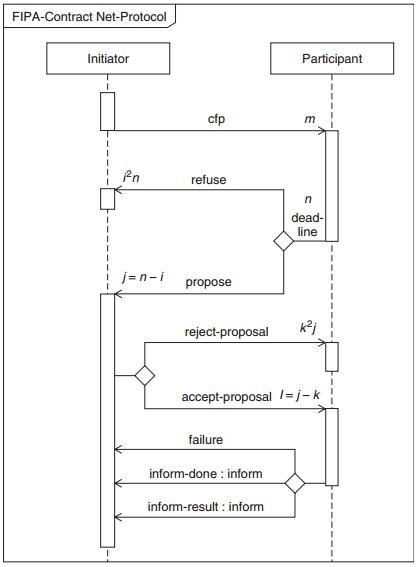
\includegraphics[scale=0.5]{figuras/contract-net-sequence_diagram.png}
    \caption{Protocolo de interação \textit{FIPA-Contract-Net}. Fonte: \citeonline[pág. 23]{developing}.}
    \label{fig:protocolo_interação_contract_net}
\end{figure}

    \item[Implementação:] a fim de demonstrar o padrão \textit{FIPA-Contract-Net}, é descrito o exemplo \textit{Book Trading} fornecido pela plataforma JADE\footnote{http://jade.tilab.com/dl.php?file=JADE-examples-4.5.0.zip (último acesso: Junho 2017)}. Todos os detalhes da implementação, configuração de ambiente e passos para execução são descritos no Apêndice \ref{appendix:contract_net}.
    
\end{description}

\section{FIPA ACL}\label{subsubsec:fipa_acl}


O FIPA-ACL baseia-se em mensagens que representam ações chamadas atos comunicativos (ou \textit{communicative acts}), como apresenta a Figura \ref{fig:communicative_acts}. São definidos ao todo um conjunto de vinte e dois atos comunicativos (Tabela \ref{tab:atos_fipa}). Alguns dos atos mais comumente usados são \textit{inform, request, agree, not understood}, e \textit{refuse} . Estes capturam a essência da maioria das formas de comunicação básica \cite[pág. 13]{developing}. Segundo \citeonline{developing}, as normas FIPA estabelecem que um agente deve ser capaz de receber qualquer \textit{communicative act}   e, no mínimo, responder com uma mensagem \textit{not-understood}, caso a mensagem recebida não possa ser processada. Com base nestes atos comunicativos, o FIPA definiu um conjunto de protocolos de interação, consistindo cada um de uma sequencia de atos comunicativos para coordenar ações multi-mensagem, como o \textit{FIPA-Contract-Net} (Seção \ref{ch:contract_net}) para o estabelecimento de acordos e vários tipos de leilões \cite[pág 14]{developing}.

\begin{figure}[h!]
    \centering
    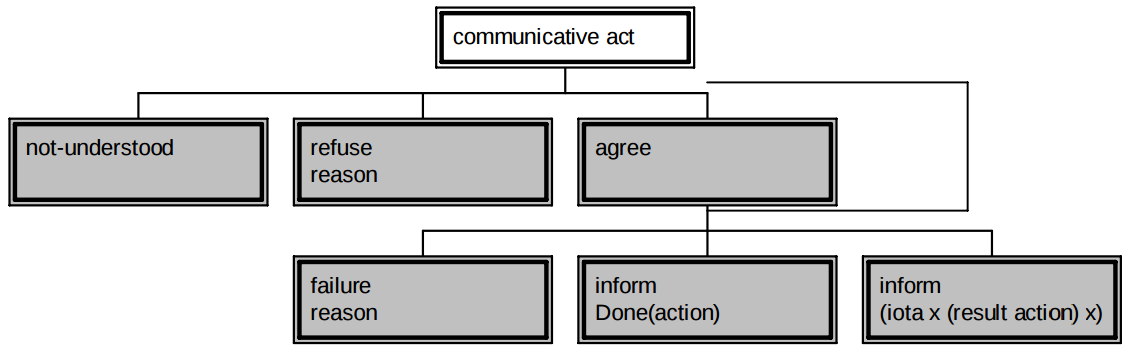
\includegraphics[scale=0.4]{figuras/communicative_acts.png}
    \caption{\textit{Communicative acts}. Fonte: \citeonline[pág. 32]{jadeguide}.}
    \label{fig:communicative_acts}
\end{figure}

% ######## init table ########
\begin{table}
 \centering \footnotesize
% distancia entre a linha e o texto
 {\renewcommand\arraystretch{1.25}
 \caption{Atos comunicativos FIPA. Traduzido. Fonte: \citeonline[pág. 19]{developing}.} \label{tab:atos_fipa}
 \begin{tabular}{ l l }
   \cline{1-1}\cline{2-2}  
    \multicolumn{1}{|p{2.750cm}|}{\textbf{FIPA \textit{communicative act}}} &
    \multicolumn{1}{p{11.700cm}|}{\textbf{Descrição}}
  \\*
  \cline{1-1}\cline{2-2}  
    \multicolumn{1}{|p{2.750cm}|}{\textit{Accept Proposal}} &
    \multicolumn{1}{p{11.700cm}|}{A ação de aceitar uma proposta previamente submetida para realizar ação.}
  \\  
  \cline{1-1}\cline{2-2}  
    \multicolumn{1}{|p{2.750cm}|}{\textit{Agree}} &
    \multicolumn{1}{p{11.700cm}|}{A ação de concordar em realizar alguma ação, possivelmente no futuro.}
  \\  
  \cline{1-1}\cline{2-2}  
    \multicolumn{1}{|p{2.750cm}|}{\textit{Cancel}} &
    \multicolumn{1}{p{11.700cm}|}{A ação de um agente informando outro agente de que o primeiro agente não tem mais a intenção de que o segundo agente execute alguma ação.}
  \\  
  \cline{1-1}\cline{2-2}  
    \multicolumn{1}{|p{2.750cm}|}{\textit{Call for Proposal}} &
    \multicolumn{1}{p{11.700cm}|}{A ação de convocação de propostas para executar uma determinada ação.}
  \\  
  \cline{1-1}\cline{2-2}  
    \multicolumn{1}{|p{2.750cm}|}{\textit{Confirm}} &
    \multicolumn{1}{p{11.700cm}|}{O remetente informa o receptor que uma dada proposição é verdadeira, onde o receptor é conhecido por ser incerto sobre a proposição.}
  \\  
  \cline{1-1}\cline{2-2}  
    \multicolumn{1}{|p{2.750cm}|}{\textit{Disconfirm}} &
    \multicolumn{1}{p{11.700cm}|}{O remetente informa o receptor de que uma dada proposição é falsa, onde o receptor é conhecido por acreditar, ou acredita que é provável que, a proposição seja verdadeira.}
  \\  
  \cline{1-1}\cline{2-2}  
    \multicolumn{1}{|p{2.750cm}|}{\textit{Failure}} &
    \multicolumn{1}{p{11.700cm}|}{A ação de dizer a outro agente que houve a tentativa de realizar uma ação, mas a tentativa falhou.}
  \\  
  \cline{1-1}\cline{2-2}  
    \multicolumn{1}{|p{2.750cm}|}{\textit{Inform}} &
    \multicolumn{1}{p{11.700cm}|}{O remetente informa o receptor que uma dada proposição é verdadeira.}
  \\  
  \cline{1-1}\cline{2-2}  
    \multicolumn{1}{|p{2.750cm}|}{\textit{Inform If}} &
    \multicolumn{1}{p{11.700cm}|}{Uma ação macro para o agente da ação para informar ao destinatário se uma proposição é verdadeira ou não.}
  \\  
  \cline{1-1}\cline{2-2}  
    \multicolumn{1}{|p{2.750cm}|}{\textit{Inform Ref}} &
    \multicolumn{1}{p{11.700cm}|}{Uma ação macro que permite ao remetente informar o receptor de algum objeto acreditado pelo remetente para corresponder a um descritor específico, por exemplo, um nome.}
  \\  
  \cline{1-1}\cline{2-2}  
    \multicolumn{1}{|p{2.750cm}|}{\textit{Not Understood}} &
    \multicolumn{1}{p{11.700cm}|}{O remetente do ato (por exemplo, \textit{i}) informa o receptor (por exemplo, \textit{j}) que percebeu que \textit{j }realizou alguma ação, mas que i não entendeu o que \textit{j} acabou de fazer. Um caso particular comum é quando i diz a\textit{ j} que \textit{i} não entende a mensagem que \textit{j} acaba de enviar para \textit{i}.}
  \\  
  \cline{1-1}\cline{2-2}  
    \multicolumn{1}{|p{2.750cm}|}{\textit{Propagate}} &
    \multicolumn{1}{p{11.700cm}|}{O remetente tem a intenção de que o receptor trate a mensagem incorporada como enviada diretamente para o receptor, e quer o receptor identifique os agentes denotados pelo descritor informado e envie a mensagem \textit{propagate} recebida a eles.}
  \\  
  \cline{1-1}\cline{2-2}  
    \multicolumn{1}{|p{2.750cm}|}{\textit{Propose}} &
    \multicolumn{1}{p{11.700cm}|}{A ação de perguntar a outro agente se uma determinada proposição é verdadeira ou não.}
  \\  
  \cline{1-1}\cline{2-2}  
    \multicolumn{1}{|p{2.750cm}|}{\textit{Proxy}} &
    \multicolumn{1}{p{11.700cm}|}{O remetente deseja que o receptor selecione agentes de destino indicados por uma dada descrição e que ele envie uma mensagem incorporada para eles.}
  \\  
  \cline{1-1}\cline{2-2}  
    \multicolumn{1}{|p{2.750cm}|}{\textit{Query If}} &
    \multicolumn{1}{p{11.700cm}|}{A ação de submeter uma proposta para executar uma determinada ação, dadas certas pré-condições.}
  \\  
  \cline{1-1}\cline{2-2}  
    \multicolumn{1}{|p{2.750cm}|}{\textit{Query Ref}} &
    \multicolumn{1}{p{11.700cm}|}{A ação de perguntar a outro agente para o objeto referido por uma expressão referencial.}
  \\  
  \cline{1-1}\cline{2-2}  
    \multicolumn{1}{|p{2.750cm}|}{\textit{Refuse}} &
    \multicolumn{1}{p{11.700cm}|}{A ação de recusar a execução de uma determinada ação, e explicando o motivo da recusa.}
  \\  
  \cline{1-1}\cline{2-2}  
    \multicolumn{1}{|p{2.750cm}|}{\textit{Reject Proposal}} &
    \multicolumn{1}{p{11.700cm}|}{A ação de rejeitar uma proposta de realização de alguma ação durante uma negociação.}
  \\  
  \cline{1-1}\cline{2-2}  
    \multicolumn{1}{|p{2.750cm}|}{\textit{Request}} &
    \multicolumn{1}{p{11.700cm}|}{O remetente solicita ao receptor que execute alguma ação. Um exemplo importante de usos do ato de \textit{request} é solicitar ao receptor que execute outro ato comunicativo.}
  \\  
  \cline{1-1}\cline{2-2}  
    \multicolumn{1}{|p{2.750cm}|}{\textit{Request When}} &
    \multicolumn{1}{p{11.700cm}|}{O remetente quer que o receptor execute alguma ação quando alguma proposição dada se torna verdadeira.}
  \\  
  \cline{1-1}\cline{2-2}  
    \multicolumn{1}{|p{2.750cm}|}{\textit{Request Whenever}} &
    \multicolumn{1}{p{11.700cm}|}{O remetente quer que o receptor execute alguma ação assim que alguma proposição se tornar verdadeira e depois cada vez que a proposição se tornar verdadeira novamente.}
  \\  
  \cline{1-1}\cline{2-2}  
    \multicolumn{1}{|p{2.750cm}|}{\textit{Subscribe}} &
    \multicolumn{1}{p{11.700cm}|}{O ato de solicitar uma intenção persistente de notificar o remetente do valor de uma referência e de notificar novamente sempre que o objeto identificado pela referência muda.}
  \\  
  \hline

 \end{tabular} }
\end{table}
